% GNUPLOT: LaTeX picture with Postscript
\begingroup
  \makeatletter
  \providecommand\color[2][]{%
    \GenericError{(gnuplot) \space\space\space\@spaces}{%
      Package color not loaded in conjunction with
      terminal option `colourtext'%
    }{See the gnuplot documentation for explanation.%
    }{Either use 'blacktext' in gnuplot or load the package
      color.sty in LaTeX.}%
    \renewcommand\color[2][]{}%
  }%
  \providecommand\includegraphics[2][]{%
    \GenericError{(gnuplot) \space\space\space\@spaces}{%
      Package graphicx or graphics not loaded%
    }{See the gnuplot documentation for explanation.%
    }{The gnuplot epslatex terminal needs graphicx.sty or graphics.sty.}%
    \renewcommand\includegraphics[2][]{}%
  }%
  \providecommand\rotatebox[2]{#2}%
  \@ifundefined{ifGPcolor}{%
    \newif\ifGPcolor
    \GPcolortrue
  }{}%
  \@ifundefined{ifGPblacktext}{%
    \newif\ifGPblacktext
    \GPblacktextfalse
  }{}%
  % define a \g@addto@macro without @ in the name:
  \let\gplgaddtomacro\g@addto@macro
  % define empty templates for all commands taking text:
  \gdef\gplbacktext{}%
  \gdef\gplfronttext{}%
  \makeatother
  \ifGPblacktext
    % no textcolor at all
    \def\colorrgb#1{}%
    \def\colorgray#1{}%
  \else
    % gray or color?
    \ifGPcolor
      \def\colorrgb#1{\color[rgb]{#1}}%
      \def\colorgray#1{\color[gray]{#1}}%
      \expandafter\def\csname LTw\endcsname{\color{white}}%
      \expandafter\def\csname LTb\endcsname{\color{black}}%
      \expandafter\def\csname LTa\endcsname{\color{black}}%
      \expandafter\def\csname LT0\endcsname{\color[rgb]{1,0,0}}%
      \expandafter\def\csname LT1\endcsname{\color[rgb]{0,1,0}}%
      \expandafter\def\csname LT2\endcsname{\color[rgb]{0,0,1}}%
      \expandafter\def\csname LT3\endcsname{\color[rgb]{1,0,1}}%
      \expandafter\def\csname LT4\endcsname{\color[rgb]{0,1,1}}%
      \expandafter\def\csname LT5\endcsname{\color[rgb]{1,1,0}}%
      \expandafter\def\csname LT6\endcsname{\color[rgb]{0,0,0}}%
      \expandafter\def\csname LT7\endcsname{\color[rgb]{1,0.3,0}}%
      \expandafter\def\csname LT8\endcsname{\color[rgb]{0.5,0.5,0.5}}%
    \else
      % gray
      \def\colorrgb#1{\color{black}}%
      \def\colorgray#1{\color[gray]{#1}}%
      \expandafter\def\csname LTw\endcsname{\color{white}}%
      \expandafter\def\csname LTb\endcsname{\color{black}}%
      \expandafter\def\csname LTa\endcsname{\color{black}}%
      \expandafter\def\csname LT0\endcsname{\color{black}}%
      \expandafter\def\csname LT1\endcsname{\color{black}}%
      \expandafter\def\csname LT2\endcsname{\color{black}}%
      \expandafter\def\csname LT3\endcsname{\color{black}}%
      \expandafter\def\csname LT4\endcsname{\color{black}}%
      \expandafter\def\csname LT5\endcsname{\color{black}}%
      \expandafter\def\csname LT6\endcsname{\color{black}}%
      \expandafter\def\csname LT7\endcsname{\color{black}}%
      \expandafter\def\csname LT8\endcsname{\color{black}}%
    \fi
  \fi
  \setlength{\unitlength}{0.0500bp}%
  \begin{picture}(9360.00,7920.00)%
      \csname LTb\endcsname%
      \put(4680,7700){\makebox(0,0){\strut{}Verhalten von $R_E$ in Abhängigkeit von $R_1$}}%
    \gplgaddtomacro\gplbacktext{%
      \csname LTb\endcsname%
      \put(1210,4290){\makebox(0,0)[r]{\strut{} 0.742}}%
      \csname LTb\endcsname%
      \put(1210,4689){\makebox(0,0)[r]{\strut{} 0.744}}%
      \csname LTb\endcsname%
      \put(1210,5087){\makebox(0,0)[r]{\strut{} 0.746}}%
      \csname LTb\endcsname%
      \put(1210,5486){\makebox(0,0)[r]{\strut{} 0.748}}%
      \csname LTb\endcsname%
      \put(1210,5885){\makebox(0,0)[r]{\strut{} 0.75}}%
      \csname LTb\endcsname%
      \put(1210,6283){\makebox(0,0)[r]{\strut{} 0.752}}%
      \csname LTb\endcsname%
      \put(1210,6682){\makebox(0,0)[r]{\strut{} 0.754}}%
      \csname LTb\endcsname%
      \put(1210,7080){\makebox(0,0)[r]{\strut{} 0.756}}%
      \csname LTb\endcsname%
      \put(1210,7479){\makebox(0,0)[r]{\strut{} 0.758}}%
      \csname LTb\endcsname%
      \put(1342,4070){\makebox(0,0){\strut{} 0}}%
      \csname LTb\endcsname%
      \put(2077,4070){\makebox(0,0){\strut{} 5}}%
      \csname LTb\endcsname%
      \put(2813,4070){\makebox(0,0){\strut{} 10}}%
      \csname LTb\endcsname%
      \put(3548,4070){\makebox(0,0){\strut{} 15}}%
      \csname LTb\endcsname%
      \put(4283,4070){\makebox(0,0){\strut{} 20}}%
      \put(176,5884){\rotatebox{-270}{\makebox(0,0){\strut{}Ersatzwiderstand $R_E$ \si{\ohm}}}}%
    }%
    \gplgaddtomacro\gplfronttext{%
      \csname LTb\endcsname%
      \put(3296,4463){\makebox(0,0)[r]{\strut{}\footnotesize{Position $1$}}}%
    }%
    \gplgaddtomacro\gplbacktext{%
      \csname LTb\endcsname%
      \put(5406,4290){\makebox(0,0)[r]{\strut{} 0.5}}%
      \csname LTb\endcsname%
      \put(5406,4822){\makebox(0,0)[r]{\strut{} 0.6}}%
      \csname LTb\endcsname%
      \put(5406,5353){\makebox(0,0)[r]{\strut{} 0.7}}%
      \csname LTb\endcsname%
      \put(5406,5884){\makebox(0,0)[r]{\strut{} 0.8}}%
      \csname LTb\endcsname%
      \put(5406,6416){\makebox(0,0)[r]{\strut{} 0.9}}%
      \csname LTb\endcsname%
      \put(5406,6947){\makebox(0,0)[r]{\strut{} 1}}%
      \csname LTb\endcsname%
      \put(5406,7479){\makebox(0,0)[r]{\strut{} 1.1}}%
      \csname LTb\endcsname%
      \put(5538,4070){\makebox(0,0){\strut{} 0}}%
      \csname LTb\endcsname%
      \put(6394,4070){\makebox(0,0){\strut{} 5}}%
      \csname LTb\endcsname%
      \put(7251,4070){\makebox(0,0){\strut{} 10}}%
      \csname LTb\endcsname%
      \put(8107,4070){\makebox(0,0){\strut{} 15}}%
      \csname LTb\endcsname%
      \put(8963,4070){\makebox(0,0){\strut{} 20}}%
    }%
    \gplgaddtomacro\gplfronttext{%
      \csname LTb\endcsname%
      \put(7976,4463){\makebox(0,0)[r]{\strut{}\footnotesize{Position $2$}}}%
    }%
    \gplgaddtomacro\gplbacktext{%
      \csname LTb\endcsname%
      \put(858,440){\makebox(0,0)[r]{\strut{} 0.72}}%
      \csname LTb\endcsname%
      \put(858,896){\makebox(0,0)[r]{\strut{} 0.73}}%
      \csname LTb\endcsname%
      \put(858,1351){\makebox(0,0)[r]{\strut{} 0.74}}%
      \csname LTb\endcsname%
      \put(858,1807){\makebox(0,0)[r]{\strut{} 0.75}}%
      \csname LTb\endcsname%
      \put(858,2263){\makebox(0,0)[r]{\strut{} 0.76}}%
      \csname LTb\endcsname%
      \put(858,2719){\makebox(0,0)[r]{\strut{} 0.77}}%
      \csname LTb\endcsname%
      \put(858,3174){\makebox(0,0)[r]{\strut{} 0.78}}%
      \csname LTb\endcsname%
      \put(858,3630){\makebox(0,0)[r]{\strut{} 0.79}}%
      \csname LTb\endcsname%
      \put(990,220){\makebox(0,0){\strut{} 0}}%
      \csname LTb\endcsname%
      \put(1813,220){\makebox(0,0){\strut{} 5}}%
      \csname LTb\endcsname%
      \put(2637,220){\makebox(0,0){\strut{} 10}}%
      \csname LTb\endcsname%
      \put(3460,220){\makebox(0,0){\strut{} 15}}%
      \csname LTb\endcsname%
      \put(4283,220){\makebox(0,0){\strut{} 20}}%
    }%
    \gplgaddtomacro\gplfronttext{%
      \csname LTb\endcsname%
      \put(3296,613){\makebox(0,0)[r]{\strut{}\footnotesize{Position $3$}}}%
    }%
    \gplgaddtomacro\gplbacktext{%
      \csname LTb\endcsname%
      \put(5538,440){\makebox(0,0)[r]{\strut{} 0.6}}%
      \csname LTb\endcsname%
      \put(5538,972){\makebox(0,0)[r]{\strut{} 0.65}}%
      \csname LTb\endcsname%
      \put(5538,1503){\makebox(0,0)[r]{\strut{} 0.7}}%
      \csname LTb\endcsname%
      \put(5538,2035){\makebox(0,0)[r]{\strut{} 0.75}}%
      \csname LTb\endcsname%
      \put(5538,2567){\makebox(0,0)[r]{\strut{} 0.8}}%
      \csname LTb\endcsname%
      \put(5538,3098){\makebox(0,0)[r]{\strut{} 0.85}}%
      \csname LTb\endcsname%
      \put(5538,3630){\makebox(0,0)[r]{\strut{} 0.9}}%
      \csname LTb\endcsname%
      \put(5670,220){\makebox(0,0){\strut{} 0}}%
      \csname LTb\endcsname%
      \put(6493,220){\makebox(0,0){\strut{} 5}}%
      \csname LTb\endcsname%
      \put(7317,220){\makebox(0,0){\strut{} 10}}%
      \csname LTb\endcsname%
      \put(8140,220){\makebox(0,0){\strut{} 15}}%
      \csname LTb\endcsname%
      \put(8963,220){\makebox(0,0){\strut{} 20}}%
    }%
    \gplgaddtomacro\gplfronttext{%
      \csname LTb\endcsname%
      \put(7976,613){\makebox(0,0)[r]{\strut{}\footnotesize{Position $4$}}}%
    }%
    \gplbacktext
    \put(0,0){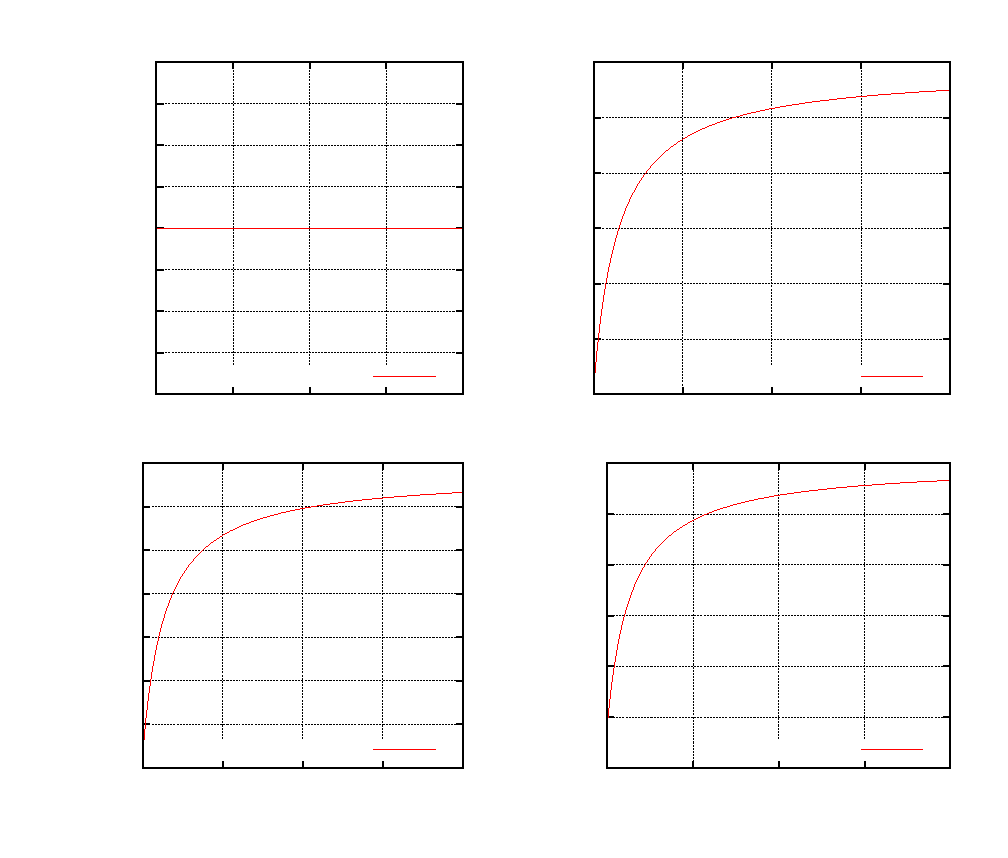
\includegraphics{./figures/wuerfel_face}}%
    \gplfronttext
  \end{picture}%
\endgroup
